\begin{savequote}[75mm]
Problems worthy

of attack

prove their worth

by hitting back. 
\qauthor{Piet Hein}
\end{savequote}

%For an example of a full page figure, see Fig.~\ref{fig:myFullPageFigure}.

\chapter{Tracking Based Point Cloud Video Segmentation}
\label{Chap:TrackingBasedSegmentation}
\lettrine[lines=3, loversize=0.3]{\textcolor{DarkBlue}S}{o far, we have presented} a 2D particle-filter based VOS method, developed a 3D point-cloud based world-model, and shown how it is possible to efficiently track within this model using particle filters. Our final task is to bridge the gap between the tracked models from the previous Chapter and the supervoxels presented in the preceding one. Connecting the two will allow us to track at the supervoxel (rather than object) level. 

The reason for tracking supervoxels rather than objects is a practical one - what we define as an ``object'' is largely dependent on context, as it is really a property of the observer, rather than the observed. By tracking supervoxels we can avoid the problem of having to make strict decisions defining object boundaries at each time step. Instead, we make ``fuzzy'' associations, where instead of a binary association decision, we instead maintain probabilities that supervoxels ``belong'' to different objects.

There are many avenues available to proceed in doing this, and which one is optimal remains an open question. In this Chapter we shall describe the avenue which we pursued, show our results, and discuss where future research should lead. We should note that the research presented in this Chapter is on-going, and while we present our current results, we hope to expand the system to be more flexible in the future.

Before we begin, it will probably be helpful if we show visually exactly what we are trying to achieve. Figure \ref{fig:TODOFIGURE} gives such an outline; the core idea is that we want to propagate supervoxels forward through time.  While the tracking we presented in the previous Chapter estimates a 6DoF pose for models in each frame, we now want to use tracked results to find a temporal association for each supervoxel. The advantage of using tracking to accomplish this is its ability to maintain object identities through occlusions, sudden movements, and other difficult situations - as well as to avoid the so-called ``aperture'' problem. 

\todo[inline]{Figure showing supervoxels, tracked models, associations to achieve segmentation}

\section{Tracked Model Representation}
The first issue that must be addressed is the ``level'' at which targets should be tracked - the object or the supervoxel level (we shall not consider tracking at the voxel level since it is computationally infeasible with current hardware). As our goal is to associate supervoxels across time, we would like to track supervoxels directly. Unfortunately, this is generally not feasible due to the ``aperture problem'' seen in neural visual fields~\cite{MarrApertureProblem}. The aperture problem deals with the fact that local motion can only be estimated perpendicular to a contour that extends beyond its field of view~\cite{shimojo1989}. In other words, determining direction of motion in a local region (without considering global features) is generally not possible - as illustrated in Figure \ref{fig:TODOFIGURE}. This means that in order to estimate motion of supervoxels, we must extend the field of view considered significantly beyond the size of the supervoxel itself; in fact, our aperture must contain the borders of the moving object in question, otherwise pairwise association of supervoxels is generally indeterminate. 

\todo[inline]{Figure showing aperture problem? Barber pole}

To avoid this problem, we must track higher level groupings - groupings that extend at least to a contour which provides a reference boundary for disambiguating motion. A natural way of doing this is to use the LCCP segmentation presented in Chapter \ref{Chap:WorldModel}, as it will expand regions up to concave boundaries. Using concave connections as references is surprisingly powerful, as it generally will differentiate objects, as well as parts of objects which can move independently (consider the case of joints in the human body). As such, we adopt a simple scheme for grouping supervoxels into tracked models; we perform LCCP segmentation on the first frame, and assign each observed segment to an independent tracker.

\section{Supervoxel-Based Particle Filters}
Tracking of the segmented models is accomplished using a bank of the correspondence-based particle filters from the previous Chapter. As our models now consist of supervoxels, so too must our observations - thus we use the supervoxels produced using the persistent scheme discussed in Chapter~\ref{Chap:WorldModel}. The observation model measures distance in a feature space of spatial distance, normals, color (in HSV space), and labels. Weights of predicted states $\mathbf{x}^j_t = [d_x, d_y, d_z, \gamma, \beta, \alpha]$ are measured by associating supervoxels from the transformed models to the observed supervoxels nearest in space. Particles are then weighted by measuring total distance in feature space, just as in (\ref{eqn:distance}), with the addition of a binary label term,
\begin{equation}
  \label{eqn:dist_labels}
    W_L =  \begin{cases} 1, & L_p = L_{p^*} \\ 
                         \frac{N_k-1}{N_k}, & L_p \neq L_{p^*} 
           \end{cases} 
\end{equation}

which results in the augmented distance function

\begin{equation} \label{eqn:augmented_distance}
  \tilde{w}^j = \sum_{1}^{\eta} \frac{1}{1 + \frac {\mu \lVert \mathbf{p}^j_{xyz} - \mathbf{p}^*_{xyz} \rVert} {R_{voxel}} +  \frac{\lambda D_c(p^j_{RGB},p^*_{RGB})}{m} +   \epsilon \lVert \mathbf{p}^j_{n_x n_y n_z} - \mathbf{p}^*_{n_x n_y n_z} \rVert + \nu  W_L}.
\end{equation}

As before, we adopt the notation $p$ for the supervoxel and $p*$ for its corresponding supervoxel in the observation.

\section{Association by Joint Energy Minimization}
The additional step that we must take to extract a full segmentation (rather than only object tracks) is to associate the observed supervoxels to the predictions coming from the particle filters. That is, we must connect the tracked outputs back to the observations, and make a per-voxel association, solving the multiple target data association problem. We do this using an energy function scheme which seeks to find a global labeling of supervoxels which minimizes our global  . To do this, we first create a list of all observed supervoxels which lie within a radius $R_{seed}$ of each predicted supervoxel coming from the particle filters (see Fig.~\ref{fig:Association}). Then we select all supervoxels which could only be associated with one possible object, associate them, and remove them from further consideration.

\begin{figure}[tb]
  \centering
  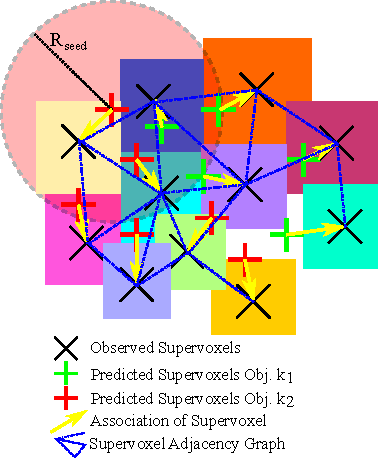
\includegraphics[scale=1.0]{figures/IROS2013/Association.pdf}
  \caption[Supervoxel Association]{Association of observed supervoxels with predicted model supervoxels using global energy.}
  \label{fig:Association}
\end{figure}

To associate the remaining observed supervoxels, we determine which objects are competing for them, and then find the predicted supervoxel from each object which lies closest to them in the feature space (using spatial location, normals, and color as in (\ref{augmented_distance})). We adopt a RANSAC-like approach, similar to \cite{EnergyBasedMultiModel}, to sample from the set of possible associations and determine a global association which best aligns the predictions to the observed supervoxels. Additionally, we use a weighted sampling strategy where the likelihood of assigning object $k$ as the label $L$ of supervoxel $p$ falls off with increasing distance from the object centroid $C_k$
\begin{equation}
 \label{eqn:WeightSampling}
 \mathcal{L}(L_p=k | C_k) = \frac{1}{C_k}.
\end{equation}

To score a set of assignments, we compute a global energy, given in~(\ref{eqn:Energy}). Each global label association $\mathcal{A}$ consists of local associations $a$ which assign an object label $k$ to each observed supervoxel $p$. The first summation term, $ \sum_{p}{\|p^*_k - p\|} $, measures error in feature space between the observed supervoxel and the closest supervoxel in its associated predicted object $p^*_k$. 

\begin{equation}
\label{eqn:Energy}
{E}_\mathcal{A} =\prod_{a\in\mathcal{A}}{\Delta_k} \left( \sum_{p}{\|p^*_k - p\|} + \lambda \sum_{(p,p')\in \mathcal{N} }\delta(L_p \not= L_{p'}) \right) 
\end{equation}

The second summation is a smoothing prior which considers the adjacency graph of observed supervoxels. For every observed supervoxel, we compare its assigned label $L_p$ to the label of all supervoxels $p'$ which lie within its adjacency neighborhood $\mathcal{N}$. We adopt the Potts model as in \cite{Boykov2001}, where $\delta(\dot)$ is 1 if the specified condition holds, and 0 otherwise, and $\lambda$ is a weighting coefficient which controls the importance given to spatial continuity of labels.

Finally, the multiplicative term $\prod_{a\in\mathcal{A}}{\Delta_k}$ controls for the expansion or contraction of object volumes through the number of observed supervoxels associated with them. $\Delta_k$ penalizes for changes in volume by increasing the energy for deviations from unity in the ratio of observed supervoxels assigned to an object $\hat{N}_k$ with the number in the object model itself $\hat{N}_k$, that is

\begin{equation}
\label{eqn:DeltaSVs}
\Delta_k = \left\{ 
  \begin{array}{l l}
    {\hat{N}_k}/{N_k} & \quad \text{if ${\hat{N}_k} \geq {{N}_k}$ }\\
    2 - {\hat{N}_k}/{N_k} & \quad \text{if $\hat{N}_k < {N}_k$}~. 
  \end{array} \right.  
\end{equation}

Once the energy arrives at a stable minimum, we extract the resulting association of observed supervoxels to predicted results, and use them to update the tracked models.

\begin{figure*}[!ht]
  \centering
  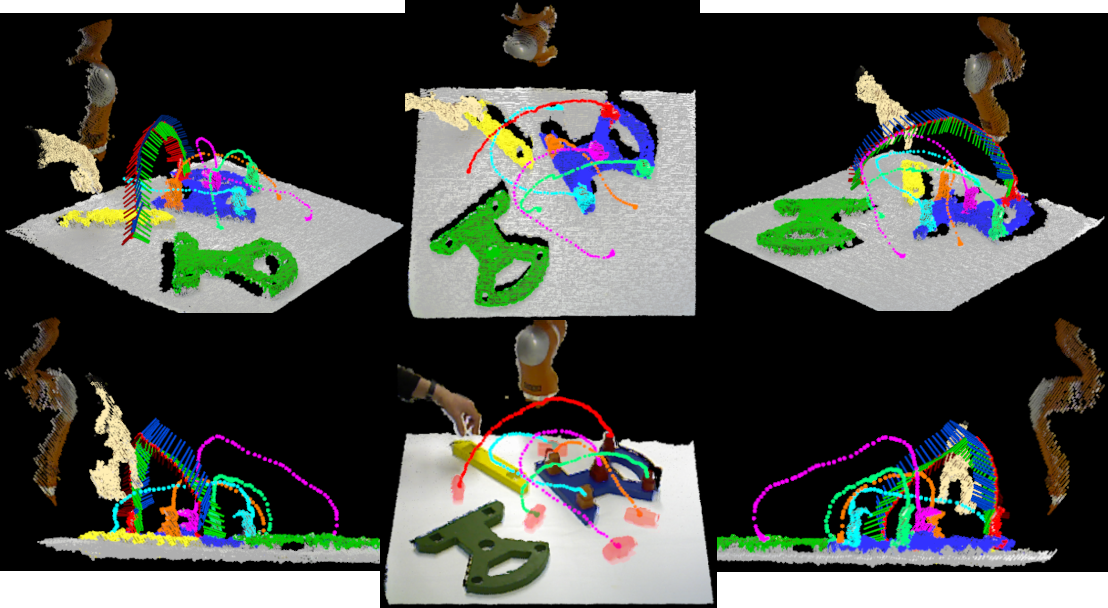
\includegraphics[width=\linewidth]{figures/IROS2013/TrajectoriesNew.pdf}
  \caption[Cranfield Tracking Results]{Result of tracking and segmentation on Cranfield scenario from different views. Here the tracks are shown as dots of the color of the tracked label for each timestep. Initial locations of the pegs are shown in the middle bottom frame as semi-transparent masks. Calculated orientation is shown for the red peg with a set of axes every second time-step; these axes show pose in a frame relative to the start. }
  \label{fig:Trajectories}
\end{figure*}

\section{Alignment and Update of Models}
The joint energy minimization results in a global association $\mathcal{A}$ which assigns observed supervoxels to tracked objects. In order to use this to update the object models, we determine a transform which aligns it to the internal representation stored by the particle filter. As an initial guess, we use the inverse of the predicted state, and then use an iterative closest point \cite{ICPChetverikov} procedure to refine the transform such that the set of observed supervoxels best aligns with the model prior. We then replace the model prior with the new observed supervoxels. 

As a final step, we use the refined transform to update the states of the particles. To do this, we shift each particle $x_i$ towards the refined state $\hat{x}$, weighting the importance given to the refined state by a constant factor $\epsilon$

\begin{equation}
\label{eqn:PFUpdate}
x'_{i \in L} = (1-\epsilon) x_i + \epsilon \hat{x}~.
\end{equation}

For this work, we found that an $\epsilon$ of $0.5$ effectively removes noise (jitter) introduced by the replacement of the tracked model. Additionally, we correct the internal motion model of the particle filters to correspond to the new updated state.

\section{Experimental Results}
In order to demonstrate the usefulness of the proposed method, in this Section we first provide results from two successful applications. Both applications use the Cranfield scenario \cite{collins1984development} as in the previous chapter. Figure~\ref{fig:Trajectories} show the results of tracking and segmentation (only the pegs are shown in Figure~\ref{fig:Trajectories} to avoid clutter) using our Cranfield pieces. It can be seen that the algorithm is able to successfully extract full segmentation throughout the video.

%%%%%%%%%%%%%%%%%%%%%%%%%%%%%%%%%%%%
\subsection{Imitation of Trajectories for Robot Manipulation}
\begin{figure}[!tb]
  \centering
  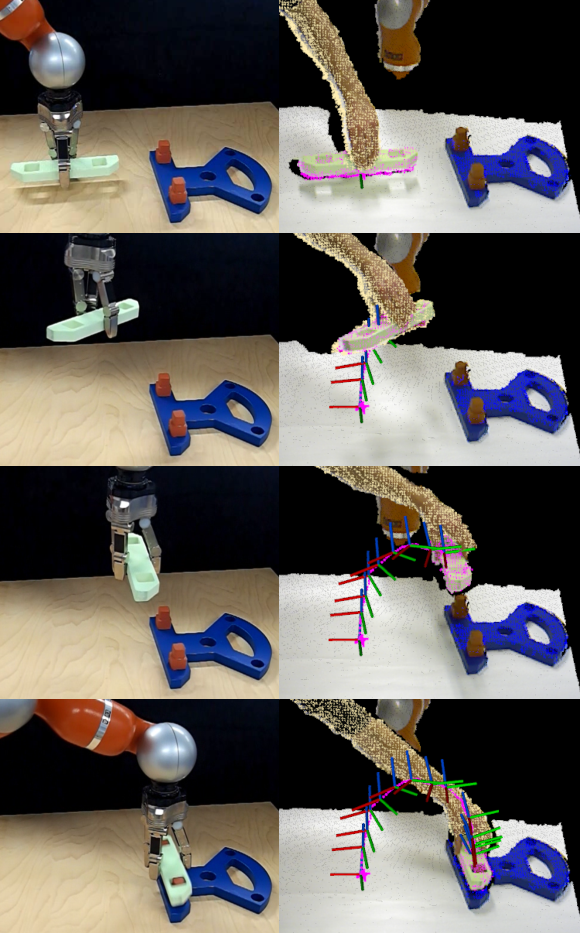
\includegraphics[scale=0.84]{figures/IROS2013/RobotImitation.pdf}
  \caption[Trajectory Imitation]{Kuka LWR arm imitating trajectory and pose learned from tracked human demonstration.}
  \label{fig:Imitation}
\end{figure}
The standard way of teaching robots to perform human-like actions is imitation learning, also called programming by demonstration \cite{Billard2008,Argall2009}. There are several ways to demonstrate movements: 1) recording movements in joint-space (joint angles) or target-space (Cartesian space) by ways of a motion capture device (requires putting markers on human body), 2) using kinaesthetic guidance (guiding a robot's movements by a human hand), or 3) via teleoperation (controlling a robot via joystick). The only way to obtain motion trajectories from human observation in a "non-invasive" procedure is by using stereo vision \cite{Hecht2009}, however, usually it is model based. The tracking algorithm we have presented here can be used as an alternative method to obtain motion trajectories (in Cartesian space) in a model-free way. 

To demonstrate this, we applied our tracking algorithm to obtain human motion trajectories in Cartesian space including orientation of manipulated object (in total six DoFs). We tested it using a recording of the Cranfield scenario where, first, we let a human demonstrate the action and then reproduced it using a KUKA Light Weight Robot (LWR) arm \cite{kuka}. Specifically, here we imitate a human putting the separator block on the pegs. To generate trajectories for the robot from human demonstrations, we used a modified version of Dynamic Movement Primitives \cite{Ijspeert2002,Ijspeert2013} (DMP) and learning method as described in \cite{Kulvicius2012}. We used Cartesian impedance control and, thus, generated six DMPs (three for motion of the end-effector in Cartesian space and three for orientation of the hand) based on trajectories obtained from the tracking algorithm. Here we used 100 equally spaced kernels with width $\sigma=0.05$ for each dimension (for more details please refer to \cite{Kulvicius2012}).
 As demonstrated in Fig.~\ref{fig:Imitation} and the supplementary video, trajectories obtained by the proposed tracking algorithm are sufficiently accurate to allow reproduction of the human motion.

%%%%%%%%%%%%%%%%%%%%%%%%%%%%%%%%%%%%

\subsection{Semantic Summaries of Actions}
\todo[inline]{Need to show results on Eren's action recordings instead, but how to show it makes a difference. Maybe use it to do object classification at the end based on what the tracked action was? Or just say we generate SECs without needing object models.}

A fundamental task for intelligent autonomous robots is the problem of encoding long chain manipulations in a generic way, for use in tasks such as learning and recognition. As a demonstration of the usefulness of the proposed tracking framework, we use a recently introduced novel Semantic Event Chain (SEC) approach \cite{Aksoy11} which converts each segmented scene to a graph: nodes represent segment (i.e. object) centers and edges indicate whether two objects touch each other or not. By using an exact graph matching technique the SEC framework discretizes the entire graph sequence into decisive main graphs. A new main graph is identified whenever a new node or edge is formed or an existing edge or node is deleted. Thus, each main graph represents a “key frame” in the manipulation sequence. Figure~\ref{fig:SECGraphs} shows a few detected sample key frames from the long Cranfield action. While the complete action has in total 1453 frames, the SEC representation reduces it to just 35 key frames, each of which represents a topological change in the scene.

\begin{figure*}[ht!]
  \centering
  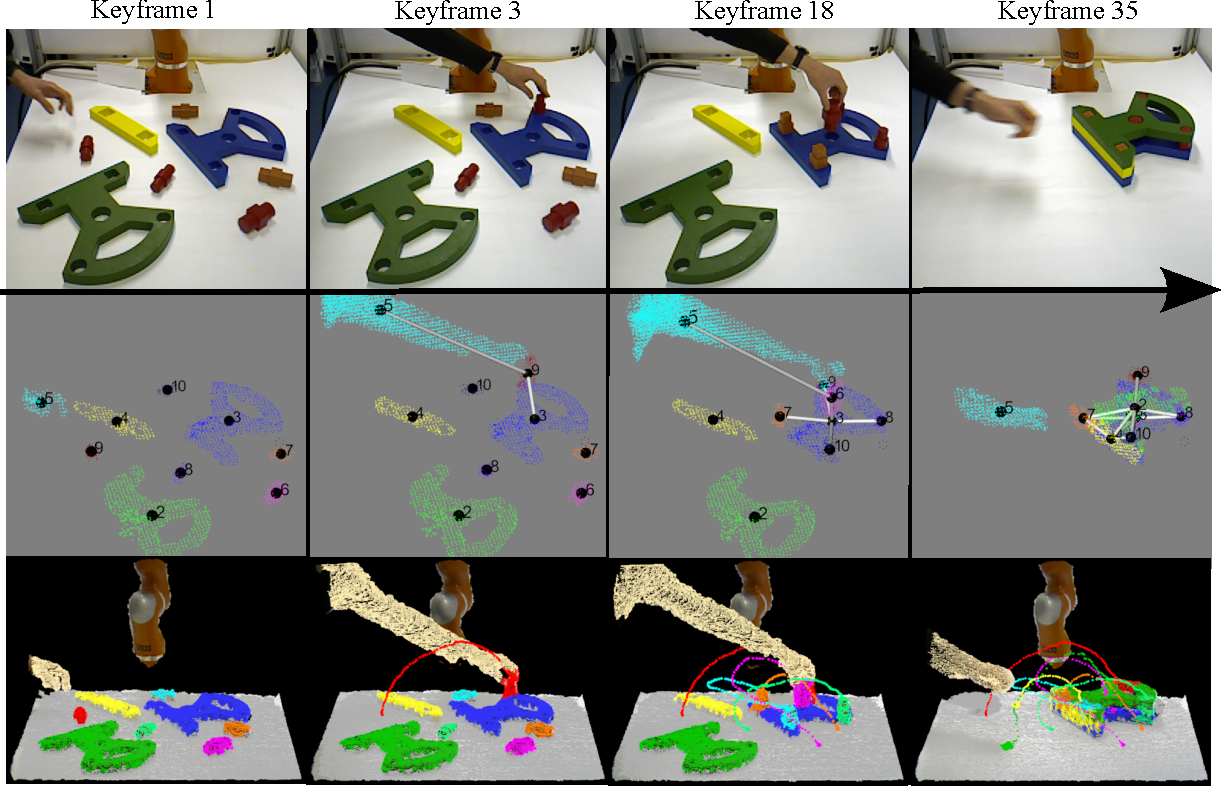
\includegraphics[width=\linewidth]{figures/IROS2013/SECKF.pdf}
  \caption[Cranfield Key Frames]{A few example key frames extracted from the long Cranfield action. Numbered nodes represent interacting objects, while edges show touching relations between objects. Each keyframe represents a topological change in the scene - here we show 4 of the 35 keyframes.}
  \label{fig:SECGraphs}
\end{figure*}